\documentclass[10pt,a4paper]{article}
\usepackage[utf8]{inputenc}
\usepackage{amsmath}
\usepackage{amsfonts}
\usepackage{amssymb}
\usepackage{makeidx}
\usepackage{graphicx}
\usepackage[left=2cm,right=2cm,top=2cm,bottom=2cm]{geometry}
\author{Miguel Angel Xamie Diaz Fuentes/Jimenez Cortes Raul}

\begin{document}
\begin{center}
\begin{LARGE}
\textbf{INGENIERÍA MECATRÓNICA}\\
\end{LARGE}
{\large Sistemas Eletrónicos De Interfaz}\\

\begin{figure}[hbtp]
\centering

\includegraphics[scale=0.80]{UPZMG_Mecatr_nica.png}
\end{figure} 

\begin{center}
\begin{LARGE}
EV2-6-Construir un amplificacion con conexion Darlington
\end{LARGE}
\end{center}

\begin{Large}
\textbf{Alumno}
\\\textit{Miguel Angel Xamie Diaz Fuentes\\Raul Jimenez Cortez}
\textbf{\\Maestro}
\\\textit{Morán Garabito Carlos Enrique}
\textbf{\\Fecha de Entrega}
\\\textit{08/11/2019}
\textbf{\\Grupo}
\\\textit{4-B}\\
\textbf{Período Cuatrimestral}\\
\textit{2019-Septiembre-Diciembre}
\\
\end{Large}

\end{center}

\footnote{Universidad Politécnica De La Zona Metropolitana De Guadalajara} 

\newpage

\subsection*{Marco teórico}
\textbf{Transistor Darlington}\\

En electrónica, el transistor Darlington es un dispositivo semiconductor que combina dos transistores bipolares en una configuración tipo Darlington en un único dispositivo a veces llamado par Darlington. Esta conexión permite que la corriente amplificada por el primer transistor ingrese a la base del segundo transistor y sea nuevamente amplificada.

La configuración originalmente realizada con dos transistores separados fue inventada por el ingeniero de los Laboratorios Bell, Sidney Darlington quien solicitó la patente el 9 de mayo de 1922. La idea de colocar dos o tres transistores sobre un chip fue patentada por el ingeniero Darlington, sin embargo, no fue así con la idea de colocar un número arbitrario de transistores sobre un mismo chip, que originaría la idea moderna de circuito integrado.\\
\begin{figure}[hbtp]
\centering
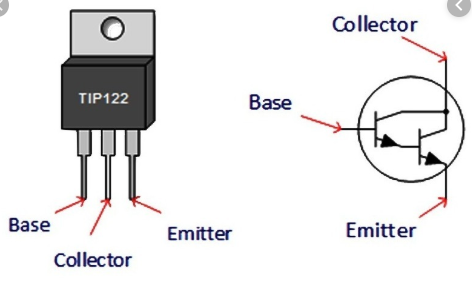
\includegraphics[scale=0.5]{1.PNG}
\caption{Transistor Darlington }
\end{figure}\\




\textbf{Comportamiento}\\
Un transistor Darlington se comporta como un transistor ordinario, es decir, posee base, colector y emisor y puede ser considerado como un único transistor con una ganancia de corriente equivalente Darlington. Generalmente suele considerarse que la ganancia de un transistor Darlington es aproximadamente el producto de las ganancias de los transistores que lo componen.\\
\begin{figure}[hbtp]
\centering
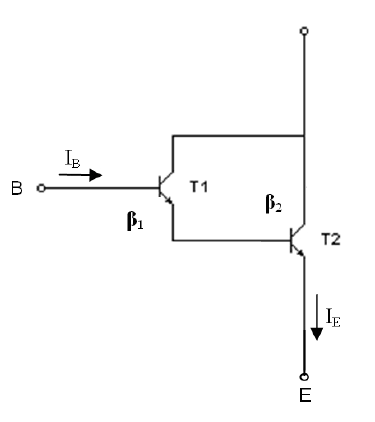
\includegraphics[scale=0.3]{2.PNG}
\caption{Comportamiento}
\end{figure}

\footnote{Universidad Politécnica de la Zona Metropolitana de Guadalajara}

\newpage
\section{Materiales}
\begin{itemize}
\item Relevadores 5V / 12V
\item Protoboard
\item LED's 
\item Transitor Darlington TIP112
\item Optoacopladores 4N25
\item Push button
\item Cable para protoboard
\item Resistencias variadas
\item Fuente de alimentación para 5V, 12V y 24V
\item Caimanes 
\item Diodos 
\item LDR
\item Relevador industrial 24V
\end{itemize}

\footnote{Universidad Politécnica de la Zona Metropolitana}

\newpage
\section{Desarrollo}
\textbf{Activación del Darlington mediante Arduino y Relevador}
Para este circuito debemos utilizar el circuito de la práctica 2: \\


\centering
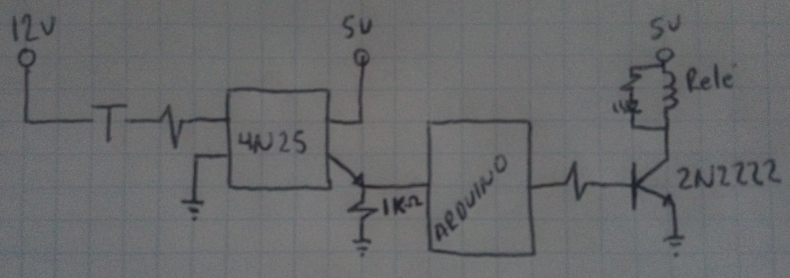
\includegraphics[scale=0.4]{3.PNG}


Pero para eso cambiamos la resistencia y el Transistor 2N2222 por el Darlington en nuestro caso TIP112, como se muestra en el siguiente circuito: \\

\centering
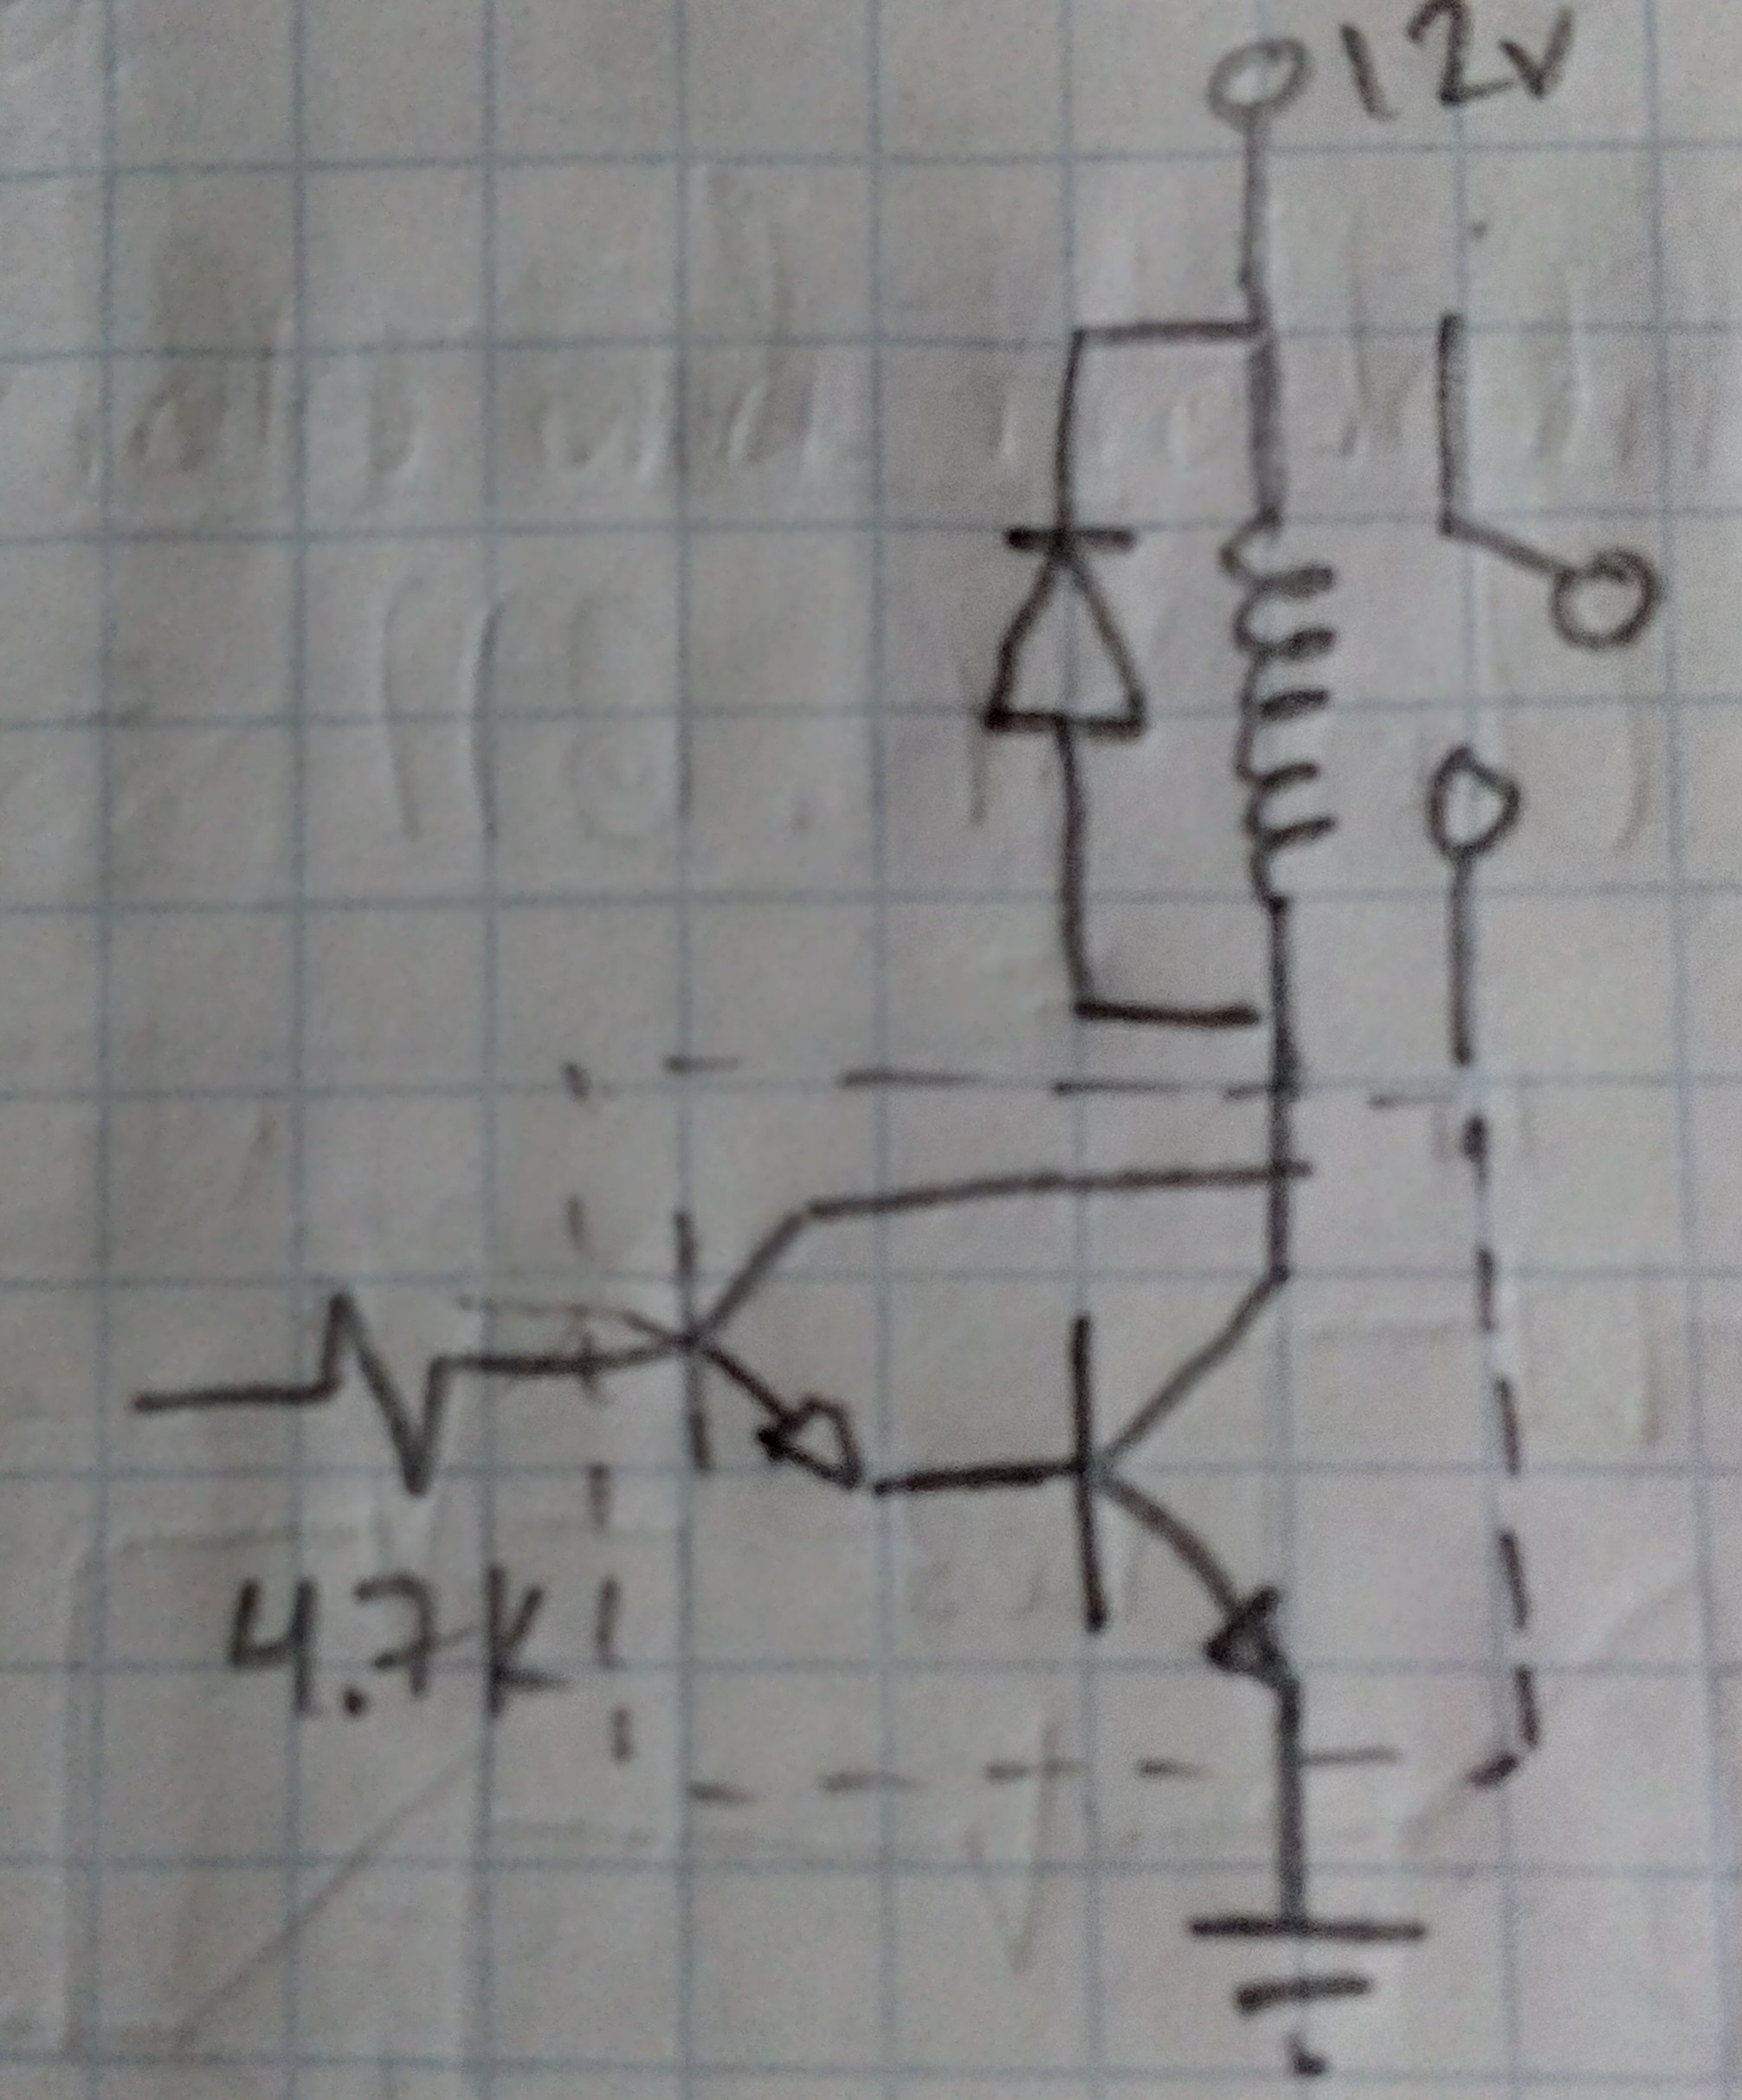
\includegraphics[scale=0.05]{4.jpg}


Despues de eoso armamos el circuito en el protoboard, quedando de la siguiente manera:\\

\centering
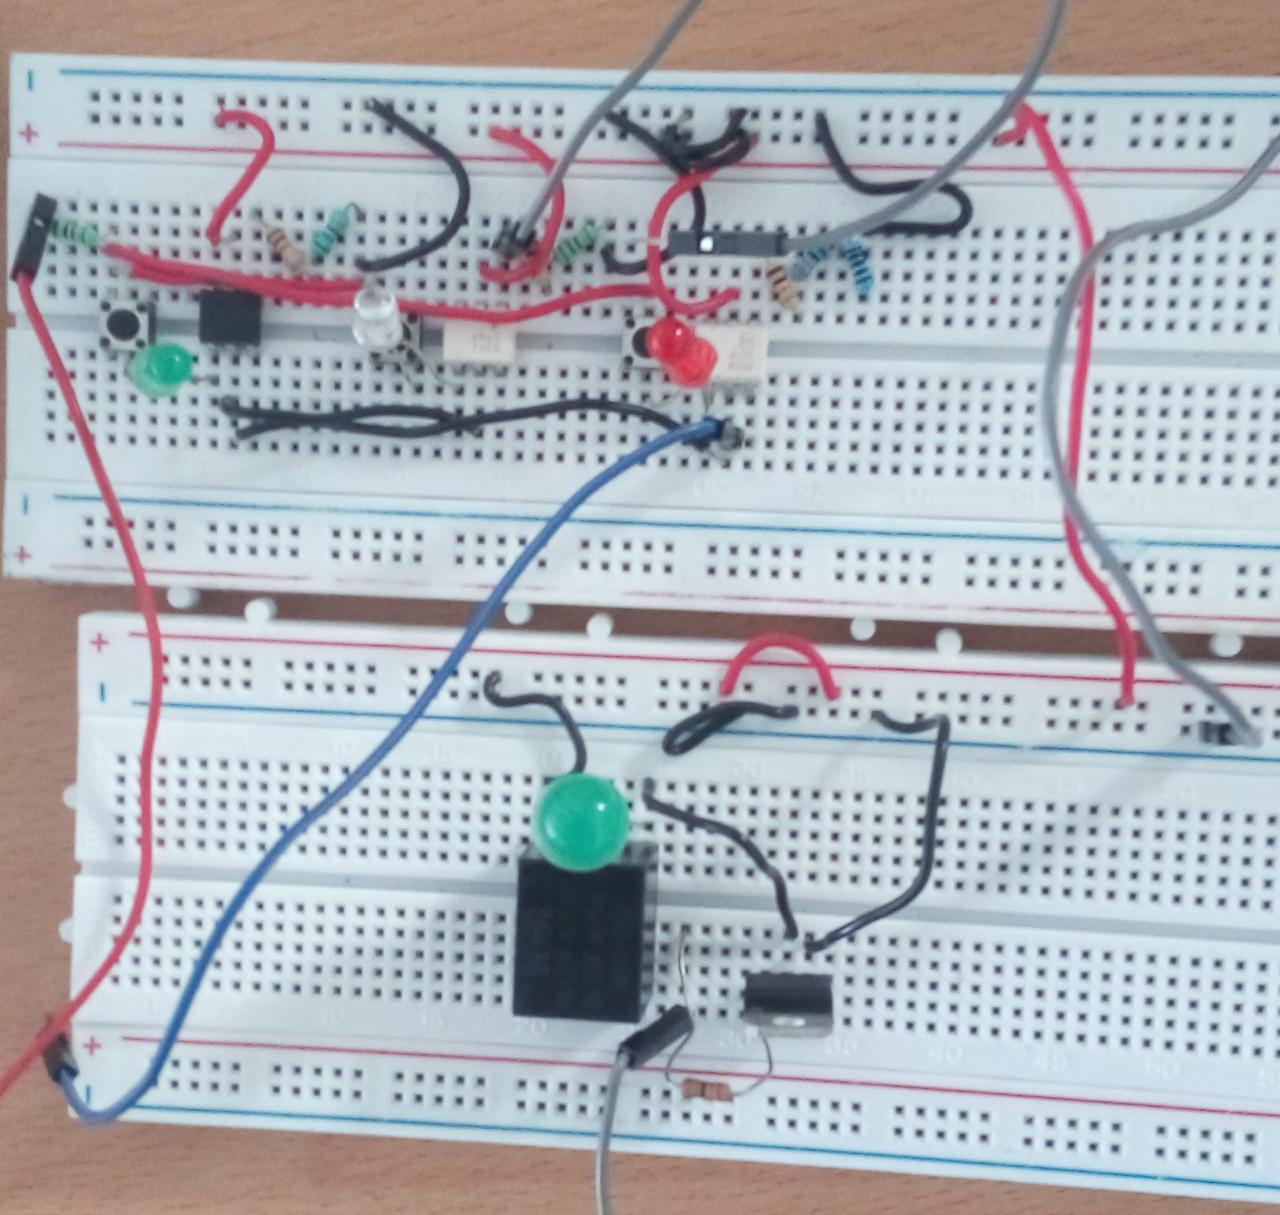
\includegraphics[scale=0.12]{5.jpeg}\\


Una vez ya armado vamos a conectar nuestras fuentes de alimentación para la activación del Darlington, teniendo una fuente de 5V para los Optoacopladores, 12V para los push button y 5V para el relavador, que puedes utilizar el mismo que utilizaste para los Optoacopladores, teniendo como resultado la activación del relevador con el darlington, mediante el arduino y código de arduino. Encendiendo el relevador y el LED para determinar que se está activando. 

\footnote{Universidad de la Zona Metropolitana de Guadalajara}

\newpage
\textbf{Activación del Darlington para activar Relevador Industrial 24V}
Para esta parte de la práctica tenemos que sustituir el relevador 5V por el relevador industrial 24V, efectivamente tenemos que también sustituir la fuente de alimentación porque si la dejamos así no nos funcionará, revisa bien tus conexiones para que todo esté correctamente para asi no quemar ningun componente u hacer un corto circuito.\\

Una vez echo esto debemos agregar un despeje para poder activar el Darlington, conectando otro negativo de otra fuente a la tierra de mis conexiones.\\


\centering
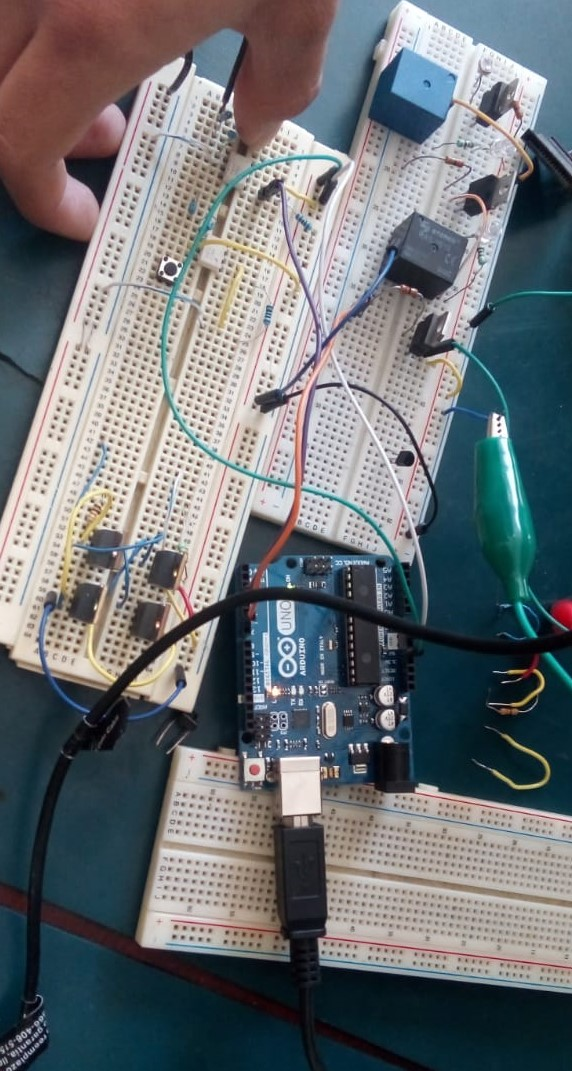
\includegraphics[scale=0.3]{6.jpeg}\\


Conectando las fuentes y asi activando el push button y esto es lo que sucede: \\


\centering
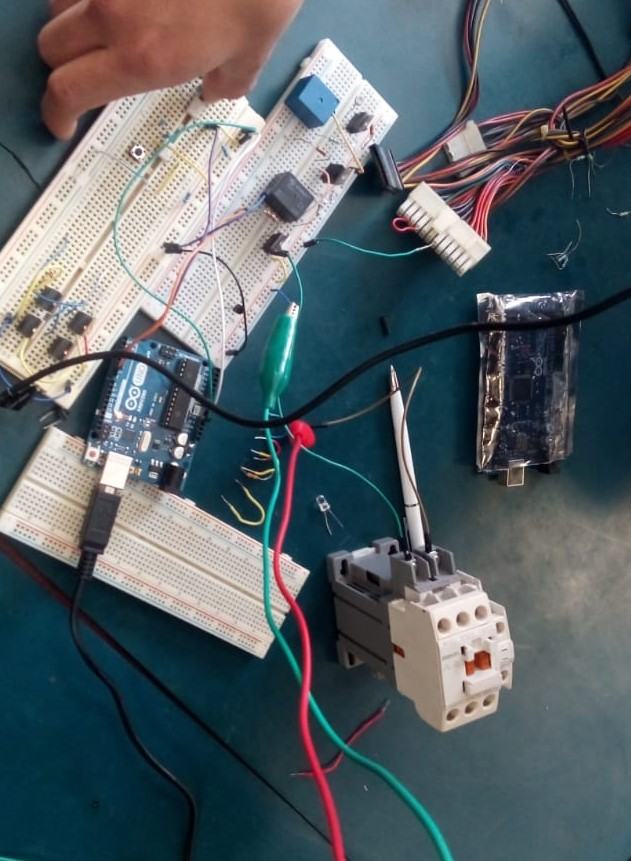
\includegraphics[scale=0.3]{7.jpeg}
\\

Observamos que el relevador industrial se activa mediante el Darlington y 24V dados por una fuente de alimentación.

\footnote{Universidad Politécnica de la Zona Metropolitana de Guadalajara}
 
\newpage
\textbf{Activación del Darlington mediante un LDR}\\
Teniendo el siguiente circuito vamos a lograr encender un Led mediante un LDR:\\

 \centering
 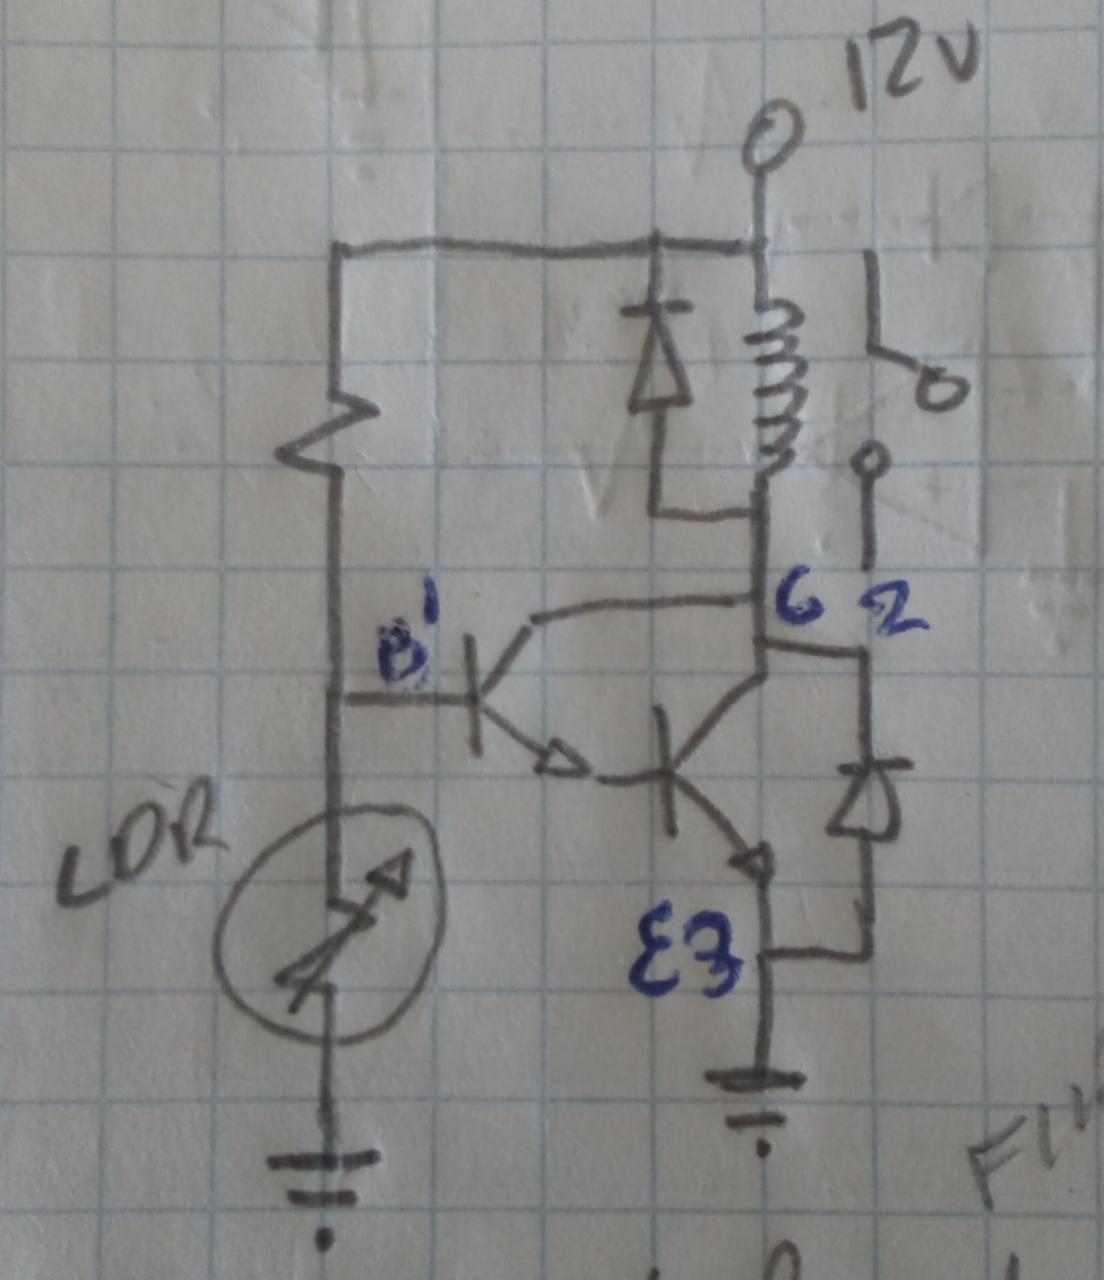
\includegraphics[scale=0.1]{8.jpeg}\\

armamos el ircuito en protoboard para poder ver el funcionamiento y la activación del Darlington, quedando el circuito armado: \\

\centering
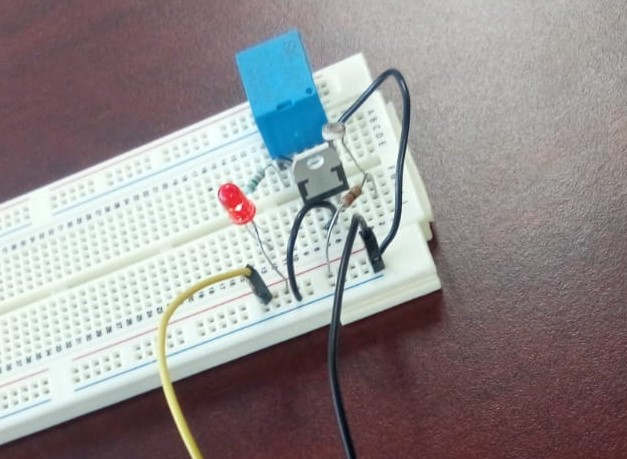
\includegraphics[scale=0.4]{9.jpeg}\\

Conectamos la fuente de voltaje en 5V y observamos lo que ocurre: \\


\centering
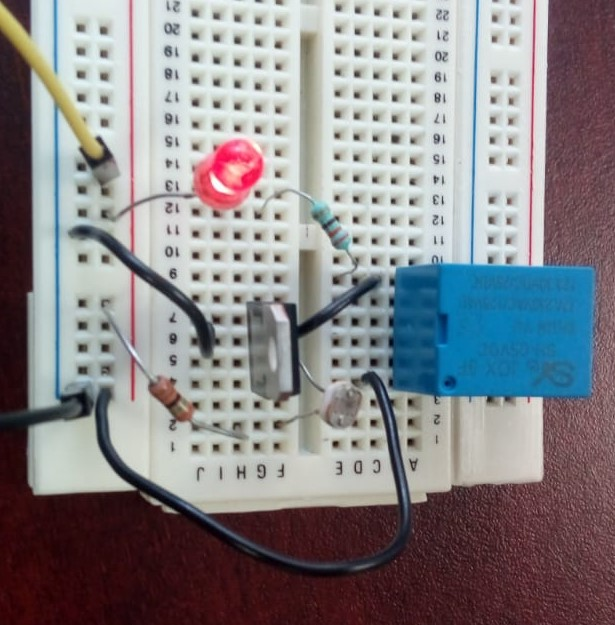
\includegraphics[scale=0.4]{10.jpeg}\\

\footnote{Universidad Politécnica de la Zona Metropolitana de Guadalajara}

\newpage
 Observamos que el LED enciende y el relevador se activa, ahora lo único que debemos de hacer es taparle la luz para que se desactive y se apague el LED, como se muestra a continuación: 

 \centering
 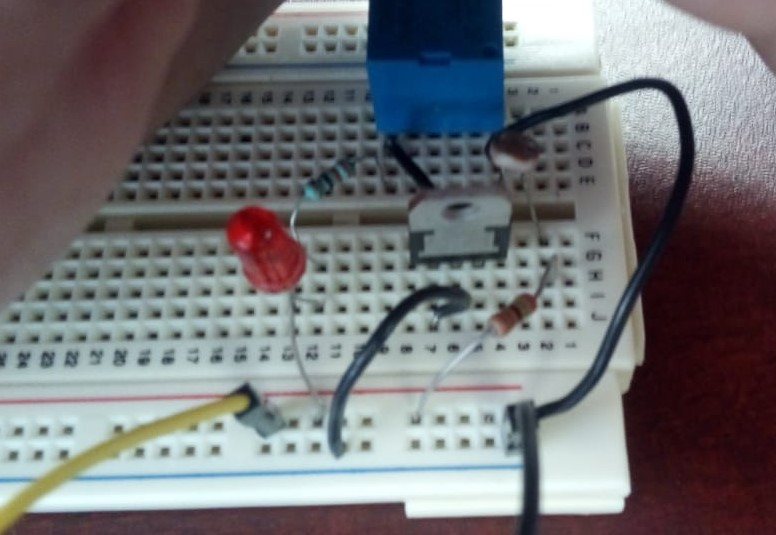
\includegraphics[scale=0.4]{11.jpeg}

 
\section{Conclusiones}
En esta práctica se comprendio cada parte que hace el reley indutrial el cual le metimos 24 volts para asi ver su funcionamiento y estar activandolo a travez de los push button conjunto el arduino, tambiren la ldr su funcion es activarse a travez de la iluminacion ya que asi activa tambien el relevador de 5v cuando se tap el ldr y cuando se destapa enciende el led asi conclimos con esta pratica el cual no hubo complicacion alguna.


\footnote{Universidad Politécnica de la Zona Metropolitana de Guadalajara}

\newpage
\section{Referencias bibliográficas}
\footnote{Universidad Politécnica de la Zona Metropolitana de Guadalajara}



\end{document}